% ---------------------------------------------------------------------------
% IEEE conference build.  Compile with:
%     tectonic -X compile main.tex --outdir .
% The body is shared verbatim with ../springer/main.tex; only this wrapper
% differs.
% ---------------------------------------------------------------------------
\documentclass[conference]{IEEEtran}
\IEEEoverridecommandlockouts

\usepackage{graphicx}
\usepackage{booktabs}
\usepackage{amsmath}
\usepackage{amssymb}
\usepackage{siunitx}
\usepackage{microtype}
\usepackage{cite}
\usepackage[hidelinks]{hyperref}

\graphicspath{{../shared/generated/}}

% siunitx v3 dropped \degree; every bare (non-\si) use in the body is in math
% mode.
\providecommand{\degree}{^{\circ}}

% IEEEtran is two-column: a "wide" float must span both columns.
\newenvironment{wfigure}{\csname figure*\endcsname}{\csname endfigure*\endcsname}
\newenvironment{wtable}{\csname table*\endcsname}{\csname endtable*\endcsname}
\newcommand{\tabscale}{\scriptsize}

% IEEEtran appends its own colon to a run-in \paragraph; adding a period too
% renders as "Mechanism.:".
\newcommand{\para}[1]{\paragraph{#1}}

% The shared body uses natbib's \citep; IEEEtran uses plain \cite.
\providecommand{\citep}[1]{\cite{#1}}

% Every experimental number in the prose is a macro; see the header comment
% in shared/generated/macros.tex for its provenance and evidence grade.
% ---------------------------------------------------------------------------
% Numeric macros used by shared/body.tex. Every instance below was re-verified
% against its primary source (a committed report/test file, or the dated prose
% in the module that ships it) on \AsOf{} -- not copied from research/research.md
% or CLAUDE.md, which is where the catalogue entries originate but which this
% paper treats as a pointer, not a source. Provenance is grouped by instance
% number, matching research/research.md's numbering (I.1, I.2, ... refer to
% that catalogue's 1.1, 1.2, ...).
%
% Evidence grade is noted per group:
%   [ARTIFACT]  a committed report/data file or a currently-passing test
%               reproduces the number on demand.
%   [DATED]     a live, single-run measurement recorded with its date in a
%               module docstring or work log, re-runnable from a named script
%               but with no stored output committed. Cited as of that date,
%               not as a standing fact.
% ---------------------------------------------------------------------------

\newcommand{\NInstances}{11}
\newcommand{\AsOf}{2026-09-09}

% --- I.4: mixed-cadence aggregation [ARTIFACT] ---
% backend/tests/test_download_cadence.py:50-80,
% test_an_hourly_field_joined_against_a_daily_one_is_a_daily_mean (passing).
% The 20.0/23.0 pair is the test's own constructed scenario (amplitude 3.0
% around a 20.0 mean, sampled at 00:00); the fixed code returns 20.0.
\newcommand{\CadMean}{20.0}
\newcommand{\CadInstant}{23.0}
\newcommand{\CadAmplitude}{3.0}
\newcommand{\CadCurrentSpeed}{1.0}

% --- I.5: circular variables [ARTIFACT for i-iii, mixed for iv] ---
% (i)/(ii) backend/services/field_sampling.py (angular sampler, angular_difference),
% backend/tests/test_field_sampling.py (passing).
\newcommand{\CircReverse}{180}
% (iii) backend/forecasting/grid_predictor.py:508-514, comment naming the
% historical shipped value directly; regression test in tests/test_derived.py.
\newcommand{\CircLegendBug}{400}
% (iv) backend/forecasting/derived.py's own docstring: a 5-degree veer across
% north trains as -355 under target_mode: delta. [DATED, in-code prose]
\newcommand{\CircDeltaVeer}{5}
\newcommand{\CircDeltaCross}{-355}

% --- I.7: Hampel outlier filter [DATED throughout; no stored report] ---
% backend/forecasting/config.py, forecasting/README.md, docs/features/forecasting.md
% all state this; backend/forecasting/preprocessing.py:161's own comment gives
% the denominator as 367, not the 365 the docs round it to -- used here since
% it is closest to the code that produced the count.
\newcommand{\HampelFlagLow}{5}
\newcommand{\HampelFlagHigh}{12}
\newcommand{\HampelZeroMAD}{74}
\newcommand{\HampelWindow}{367}
\newcommand{\HampelSkillWith}{0.138}
\newcommand{\HampelSkillWithout}{0.202}

% --- I.8: eddy detector [ARTIFACT for mechanism tests; DATED for the count] ---
% backend/services/eddies.py (polarity, antimeridian, white-noise-floor all
% covered by passing tests); count/timing from DONE.md's 2026-08-15 entry, a
% live snapshot of the current-field state, not a fixed model artifact.
\newcommand{\EddyCount}{2{,}097}
\newcommand{\EddyCyclonic}{954}
\newcommand{\EddyAnticyclonic}{1{,}143}
\newcommand{\EddyRadius}{55}
\newcommand{\EddyPassTime}{0.1}
\newcommand{\EddyLoopTime}{37}

% --- I.9: bilinear resampling over a NaN-holed grid [ARTIFACT] ---
% backend/services/field_sampling.py's own module docstring states this
% directly, and backend/tests/test_forecast_grid.py::
% test_the_painted_edge_reaches_halfway_to_the_first_land_cell pins the fixed
% boundary geometrically (passing).
\newcommand{\BilinearStaircaseKm}{110}
\newcommand{\BilinearErasedCells}{3{,}609}
\newcommand{\BilinearTotalCells}{42{,}499}
\newcommand{\BilinearErasedPct}{8.5}
% Contrast ratios are a separate, [DATED] sub-claim (docs/features/forecasting.md),
% about the forecast-tile colour ramp rather than the coverage-field fix itself.
\newcommand{\BilinearContrastLow}{1.13}
\newcommand{\BilinearContrastHigh}{1.27}

% --- I.1: softmax ensemble weighting ---
% [DATED, commit 7acf907, 2026-08-13] -- the numbers research.md's catalogue
% entry quotes. The model has since been retrained; these are cited as a
% point-in-time measurement, not a standing fact (see body.tex's discussion of
% why this instance's own evidence illustrates the paper's thesis).
\newcommand{\EnsMaxentCVOld}{0.619}
\newcommand{\EnsLGBMCVOld}{0.826}
\newcommand{\EnsMaxentVoteOld}{27}
\newcommand{\EnsPropScoreOld}{0.694}
\newcommand{\EnsBestMemberOld}{0.788}
\newcommand{\EnsSoftmaxScoreOld}{0.792}
\newcommand{\EnsBoyceOldBefore}{0.936}
\newcommand{\EnsBoyceOldAfter}{0.905}
% [ARTIFACT, re-verified \AsOf{}] machine_learning/reports/fish_habitat_summary.json
% and fish_habitat_holdout.csv, read directly.
\newcommand{\EnsMaxentCVNow}{0.689}
\newcommand{\EnsLGBMCVNow}{0.825}
\newcommand{\EnsRFCVNow}{0.821}
\newcommand{\EnsWeightLGBMNow}{50.2}
\newcommand{\EnsWeightRFNow}{46.5}
\newcommand{\EnsWeightMaxentNow}{3.3}
\newcommand{\EnsHoldoutEnsembleNow}{0.8554}
\newcommand{\EnsHoldoutBestNow}{0.8564}

% --- I.2: global vs regional habitat model ---
% [ARTIFACT] Headline numbers only, cross-checked directly against
% machine_learning/reports/global_vs_regional_habitat.csv on \AsOf{}; full
% mechanism (MESS, SHAP, ablation) is the companion paper
% research/papers/global_vs_regional/, cited rather than re-derived here.
\newcommand{\GvrTSSRegion}{0.798}
\newcommand{\GvrTSSGlobal}{0.448}
\newcommand{\GvrDataMultiple}{64.7}
\newcommand{\GvrNRegionalTrain}{1{,}902}
\newcommand{\GvrNGlobalTrain}{123{,}104}
\newcommand{\GvrMESSGlobal}{1.24}
\newcommand{\GvrMESSRegion}{9.04}

% --- I.11: corroboration needs a control arm [DATED, 2026-08-17] ---
% backend/services/upwelling.py's own module docstring; control_cool_fraction
% as a returned field is [ARTIFACT] (services/upwelling.py:377-379); the
% eastern-boundary/hemisphere regression is a passing test
% (backend/tests/test_upwelling.py).
\newcommand{\UpwellFavor}{19.9}
\newcommand{\UpwellControl}{17.2}
\newcommand{\UpwellStrongFavor}{4.1}
\newcommand{\UpwellStrongControl}{3.9}
\newcommand{\UpwellAnomFavor}{0.91}
\newcommand{\UpwellAnomControl}{0.60}

% --- I.12: a baseline fitted on one product cannot score another ---
% [DATED throughout] backend/services/sst_anomaly.py's own module docstring,
% three separate dated attempts (2026-08-17, 2026-08-25, 2026-08-28), each
% naming its own reproduction script; no stored output file for any of them.
\newcommand{\SstWeakOISST}{0.026}
\newcommand{\SstWeakLive}{0.022}
\newcommand{\SstStrongOISST}{0.002}
\newcommand{\SstStrongLive}{-0.149}
\newcommand{\SstMeanOpen}{0.033}
\newcommand{\SstSDOpen}{0.467}
\newcommand{\SstOpenFracHalf}{14.3}
\newcommand{\SstOpenFracOne}{3.9}
\newcommand{\SstMeanCoastal}{0.131}
\newcommand{\SstSDCoastal}{0.758}
\newcommand{\SstCoastalFracHalf}{24.9}
\newcommand{\SstCoastalFracOne}{10.0}
\newcommand{\SstMatchedOISSTStrong}{-0.001}
\newcommand{\SstMatchedGLORYSStrong}{-0.051}

% --- I.13: HAB precision tracks regional base rate [ARTIFACT] ---
% machine_learning/reports/hab_early_warning_*_summary.json and the matching
% *_holdout.csv for all five regions, read directly on \AsOf{}.
\newcommand{\HabArabianBase}{0.076}
\newcommand{\HabBengalBase}{0.078}
\newcommand{\HabArabianPrecSeven}{0.202}
\newcommand{\HabBengalPrecSeven}{0.187}
\newcommand{\HabArabianLiftSeven}{0.053}
\newcommand{\HabBengalLiftSeven}{0.150}

% --- 2.5: batched spatiotemporal sampling equivalence [ARTIFACT, reproduced
% live \AsOf{}] machine_learning/marine_ml/fusion.py:358 (_BATCH_PAD_DAYS = 45);
% machine_learning/tests/test_global_sources.py::
% test_year_batched_sampling_matches_the_unbatched_path (passing); pad=0
% failure reproduced live by monkeypatching the constant and rerunning the
% test's own fixture (max abs diff on thetao = 2.9170, 2 affected rows).
\newcommand{\BatchPadDays}{45}
\newcommand{\BatchThetaoErrorNoPad}{2.92}


\begin{document}

\title{Silent, Plausible, and Signed: Eleven Measured Failure Modes in One
Operational Marine Machine-Learning Pipeline}

\author{\IEEEauthorblockN{Deepak Krishna}
\IEEEauthorblockA{\textit{MarisAI} \\
India \\
deepakkrishna2206@gmail.com}}

\maketitle

\begin{abstract}
An operational machine-learning system rarely fails by crashing; it keeps
running, produces output of the right shape and units, and looks correct. We
report \NInstances{} instances of exactly that from one running marine
data-and-modelling platform, each caught not by a failing test but by a
second, cheap check most pipelines never run: a simpler baseline, a control
arm, a hand-computed reference value, a synthetic fixture with a known
answer, or an adversarial fixture built to break the code a specific way.
None raised an exception or halted a pipeline, and every one biased its host
metric in the direction that makes the system look better, or at least
normal. We organise the eleven into three branches of \emph{how}
the failure stays hidden --- no signal survives at all; a real, correctly
computed number is licensed by convention to mean more than it does; or the
behaviour is textbook and expected, so its downstream cost is never
re-examined --- and map each instance to the specific check that caught it.
Because a paper about untrusted plausible numbers cannot itself rest on
unverified prose, we grade every instance's own evidence (a committed
artifact versus a dated, reproducible-on-demand measurement) and report two
of our own numbers caught drifting while writing this paper, including a
transcription error in a companion manuscript, as further,
unplanned instances of the same thesis.
\end{abstract}

\begin{IEEEkeywords}
software engineering for machine learning, data quality, silent failure,
technical debt, reproducibility, marine data systems
\end{IEEEkeywords}

% ---------------------------------------------------------------------------
% The manuscript body, shared verbatim by the Springer (LNCS) and IEEE
% (IEEEtran) builds. Nothing class-specific may appear in this file.
%
% Each wrapper defines, before \input-ing this:
%   \wfigure / \endwfigure   a figure spanning the full text width
%   \wtable  / \endwtable    the same for tables
%   \tabscale                the font size command tables are set at
%   \para{...}               a run-in bold paragraph heading
%   \citep{...}               mapped to \cite for the LNCS/IEEEtran builds
% ---------------------------------------------------------------------------

\section{Introduction}

An operational machine-learning system rarely fails by crashing. It keeps
running, produces output of the right shape and the right units, and looks
correct --- and the failure that matters is the one that never trips an
exception, an alert, or a test that was already passing. This paper reports
eleven such failures, each one found and fixed inside a single running
platform (marine ocean-data ingestion, forecasting, and species-distribution
and harmful-algal-bloom modelling), and each one caught not by monitoring,
not by a test that failed, but by a second, cheap check that most pipelines
never run: a comparison against a simpler baseline, a control arm, a value
computed by hand from raw data, a synthetic case with a known correct answer,
or a fixture built deliberately to break the code in a specific way. None of
the eleven raised an exception or halted a pipeline. Every one biased its
host metric in the direction that makes the system look better, or at least
look normal, than it is.

This is not a paper about one bug. It is a paper about a shape that recurs:
a system component that is individually well-tested and behaves exactly as
documented, feeding a downstream reading that is technically a real number
computed from real data, which is nonetheless the wrong number to trust for
the question being asked of it. Sculley et al.~\citep{sculley2015} named the
general phenomenon at the level of system architecture --- machine learning
systems accrue a form of technical debt largely invisible to the metrics
that are usually watched. Sambasivan et al.~\citep{sambasivan2021} documented
it at the level of organisational practice --- data problems compound
silently across a pipeline because "data work" is systematically undervalued
relative to "model work." This paper sits between those two: eleven concrete,
measured instances from one running system, each with the specific check
that caught it named and, where the evidence supports it, reproducible on
demand.

\subsection{Contributions}

\begin{enumerate}\itemsep2pt
\item \textbf{Eleven measured instances} of silent, plausible, signed-direction
failure, drawn from production code rather than constructed as illustrations,
spanning data ingestion, geometric resampling, ensemble modelling, detector
design, and cross-region evaluation.
\item A \textbf{three-branch taxonomy of how the failure stays hidden}: no
signal survives at all (\S\ref{sec:branch-a}); a real, correctly computed
number is licensed by convention to mean more than it does
(\S\ref{sec:branch-b}); or the behaviour is documented and expected, so its
downstream consequence is never re-examined (\S\ref{sec:branch-c}).
\item An explicit \textbf{mapping from each instance to the check that caught
it} (Table~\ref{tab:instances}), because "run a second, cheap check" is only
actionable advice once the check itself is named.
\item A \textbf{reproducibility ledger, applied to this paper's own claims}:
six of the eleven instances are fully backed by a committed report or a
currently-passing regression test; three combine a tested mechanism with a
headline number that is a dated, single live measurement of a state that
moves (a current field, a wind field, a just-retrained model); and two rest
entirely on a dated measurement with no committed artifact at all, each
naming the script that reproduces it and reported as of its date rather
than as a standing fact (\S\ref{sec:method}). Two of those dated numbers
were caught drifting while
writing this paper, which \S\ref{sec:discussion} reports as a further
instance of the paper's own thesis rather than an inconvenience to edit
around.
\end{enumerate}

\section{Related Work}
\label{sec:related}

\para{Technical debt in ML systems} Sculley et al.~\citep{sculley2015}
catalogue system-level hazards --- boundary erosion, hidden feedback loops,
undeclared consumers, glue code --- that accumulate in production machine
learning without tripping any single component's tests. That paper argues
at the level of system design; this one operates one level down, at the
level of a specific number a specific function returns, and asks what
second check would have shown that number to be misleading. Several of the
instances here are concrete specialisations of debt classes that paper names
only abstractly: I.9's coverage field and I.4's aggregation ordering are
both "hidden feedback" in the sense that the input's own geometry silently
determines what a downstream consumer receives.

\para{Data cascades} Sambasivan et al.~\citep{sambasivan2021} define a data
cascade as a compounding, downstream effect of a data-quality issue that is
invisible at its point of origin and surfaces far away, in high-stakes
deployment contexts. I.4 (an instantaneous sample standing in for a period
mean), 2.5 (a memory-motivated batching change that is not value-identical
to the path it replaces), and I.9 (a resampling routine that erases the
coastal band it was asked to preserve) are data cascades in exactly that
sense, with one addition: each is quantified with a specific, measured cost
--- a skill delta, an error magnitude, a cell count --- rather than reported
as a category of risk. Their interview-based methodology surfaces that data
work is undervalued across many teams; this paper's contribution is
complementary evidence of \emph{what that undervaluing costs}, itemised, in
one system where it was possible to measure.

\para{Scope} This is a single-system instance catalogue, not a general
taxonomy validated across projects, and \S\ref{sec:limitations} says so
directly. Two of the eleven instances are the headline results of dedicated
companion papers from the same codebase --- ensemble weighting (I.1) and the
global-versus-regional habitat comparison (I.2, \citep{moredata2026}) --- and
are summarised here rather than re-derived; a third companion paper
\citep{risingskill2026} establishes the persistence-baseline finding this
paper's framing extends to eleven further instances outside forecasting
alone.

\section{Method: how these were found, and how each is graded}
\label{sec:method}

\para{The five checks} Across the eleven instances, the check that surfaced
the problem falls into one of five kinds, and more than one recurs per
instance: (1) a \emph{second baseline or reference} --- scoring an ensemble
against its own best member, or a filtered series against its unfiltered
one; (2) a \emph{control arm} --- measuring a signal where it is not
expected to hold, alongside where it is; (3) a \emph{hand-computed value}
against raw data --- counting erased cells directly, or computing a
per-product dispersion by hand; (4) a \emph{synthetic fixture with a known
correct answer} --- a diurnal cycle whose true mean is known by construction,
a batching path checked against its own unbatched reference; and (5) a
fixture built \emph{deliberately to break} the code in a specific,
adversarial way --- a vortex placed on the antimeridian, a coastline placed
to the west instead of the east, a field of pure white noise. None of the
five is expensive. All five are absent by default from a pipeline whose own
tests pass and whose own output looks plausible.

\para{Evidence grading} A paper whose thesis is "the plausible number is not
the one to trust" cannot itself rest on unverified prose, and this project's
own written history already contains a caution that applies directly here:
a dated note recorded during a previous session is a claim about that
session, not a standing fact, and has been wrong before after
re-investigation. Accordingly, every instance below is marked as backed
either by a \emph{committed artifact} --- a report file or a currently
passing regression test that reproduces the number on demand, re-verified as
part of writing this paper on \AsOf{} --- or by a \emph{dated measurement}:
a single, live run recorded with its date, naming the script that would
reproduce it, with no output file committed. Six instances (I.2, I.4, I.5,
I.9, I.13, 2.5) are fully artifact-backed --- every sub-claim traces to a
report file or a currently-passing test, with nothing resting on a value
that could differ if re-measured today. Three (I.1, I.8, I.11) pair a
tested mechanism with a headline number that \emph{is} exactly that kind of
value: a live measurement of something that keeps moving --- a
just-retrained model's cross-validated score, a day's ocean-current field, a
day's wind field --- rather than a fixed model artifact. The remaining two
(I.7, I.12) rest entirely on a dated measurement, with no committed test
covering even the mechanism; two of the dated numbers across these two
groups (I.1, I.12) turned out to matter, as \S\ref{sec:discussion} reports.

\para{System} All eleven instances come from MarisAI, an ocean-data platform
combining live provider ingestion (satellite and reanalysis products), a
forecasting engine trained per-variable per-site, a detector layer (eddies,
upwelling, marine heatwaves), and offline species-distribution and
harmful-algal-bloom pipelines sharing a common feature-store spine. No
architectural detail beyond what a given instance needs is given here; the
companion papers \citep{risingskill2026,moredata2026} describe the
forecasting and habitat-modelling components respectively in full.

\section{Results: eleven instances}
\label{sec:results}

\subsection{Branch A: no signal survives at all}
\label{sec:branch-a}

In these three, the wrong answer produces no exception and, for most of the
symptoms described, nothing a bounds check would catch either --- it is a
real number in the right units, silently computed from the wrong quantity.
The one exception inside this branch is named where it occurs (I.5's colour-
scale symptom): even there, nothing stopped the pipeline, because nothing
checks a percentile against a circular domain.

\para{I.4 --- a period mean silently becomes an instantaneous sample.}
Joining an hourly product against a daily one and aggregating afterwards
substitutes the join's arbitrary matched timestamp for a period mean, with
no signal that a substitution occurred. On a synthetic \CadAmplitude{}\si{\celsius}-amplitude
diurnal cycle around a \CadMean{}\si{\celsius} mean, the 00:00 sample is exactly
\CadInstant{}\si{\celsius} --- the full amplitude away from the true daily mean, in a
signed direction fixed by what time of day the join happens to land on. A
companion defect in the same code path is non-linear: a current rotating at
a constant 1~m/s speed averages its $u$/$v$ components to $\approx 0$ before
the speed is derived, reporting \emph{slack water} for a current that never
stopped moving, unless speed is derived before the aggregation rather than
after (verified: a full daily rotation at unit speed derives to
\CadCurrentSpeed{}~m/s only when ordered this way). The fix reorders
resolution, aggregation, and merge so the coarse product's own cadence
determines the join, and a regression test builds exactly this scenario.

\para{I.5 --- a circular variable breaks at every layer that treats it as
linear.} A bearing on $[0,360)$ has the property that 359\si{\degree} and
1\si{\degree} are two degrees apart, not \CircReverse{}\si{\degree} apart ---
and every stage of a pipeline that is not built for that property gets it
wrong the same way. Naive linear interpolation of those two headings
returns \CircReverse{}\si{\degree}, the exact reverse of both inputs; this is
fixed by resampling in sin/cos space and recombining with \texttt{atan2}. A
forecast \emph{difference} needs the analogous fix, a signed veer wrapped to
$[-180,180)$, or a percentile-based colour scale computed on a circular
domain silently ships a range like \texttt{display\_max:\allowbreak{}
\CircLegendBug{}} on a field whose true maximum is 360\si{\degree}. A fourth
layer sits underneath the first three and is the one that is easy to miss
entirely: a forecasting model trained with \texttt{target\_mode: delta}
learns the \emph{numeric change} in the bearing, and a \CircDeltaVeer{}-degree
veer across north trains as \CircDeltaCross{} --- teaching the model an
enormous excursion that never physically happened, while the model still
fits, still scores, and still produces bearings in range. The fix for this
fourth layer is not a wrapping correction but an architectural one: forecast
the vector components and derive the bearing, exactly as the codebase's own
particle-advection layer already did for unrelated reasons, which is
precisely why that layer was never affected while the raster direction layer
was. This closes the gap for wind and current direction, both of which have
components to decompose into; wave direction has no such components in this
system and remains linearly trained, a disclosed, deliberate asymmetry
rather than the same open gap under a different name.

\para{2.5 --- a memory-saving batch is not automatically value-identical.}
A global point-sampling job batched by calendar year, built because the
unbatched path exhausts memory on a resource-constrained machine, looks like
a pure performance change: same inputs, same code path per batch, smaller
peak memory. It is not value-identical unless two specific details are
handled. First, source products are stamped mid-month with nearest-in-time
selection, so a point near a year boundary can have its true nearest
timestep fall in the adjacent year; without a temporal pad, a batch boundary
silently substitutes the wrong timestep. Second, one derived quantity (eddy
kinetic energy) is computed against the whole record's mean, which a
per-year batch would instead compute against that year's own mean under an
identical column name, corrupting the value while leaving its label
unchanged. With the padding at \BatchPadDays{} days, the equivalence holds
to within the batching path's own test tolerance ($10^{-6}$, relative and
absolute); reproduced directly for this paper by removing the pad and
re-running that same equivalence fixture, the maximum absolute error on one
variable (\texttt{thetao}) is \BatchThetaoErrorNoPad{}\si{\celsius},
affecting precisely the two rows that sit at a year boundary --- silent
because a batching refactor is not the kind of change anyone expects to
alter a value at all.

\subsection{Branch B: a real number, licensed to mean more than it does}
\label{sec:branch-b}

In these five, the number itself is computed correctly. What is silent is
the unlicensed step between the number and the conclusion drawn from it.

\para{I.1 --- an ensemble's own accuracy score does not certify that
combining helped.} Weighting an ensemble's members proportionally to a skill
score whose chance level is zero compresses a large quality gap into a
small weight gap. Measured 2026-08-13: MaxEnt's cross-validated true skill
statistic (TSS) of \EnsMaxentCVOld{} against LightGBM's \EnsLGBMCVOld{} ---
less than half as good on the holdout --- still drew \EnsMaxentVoteOld{}\% of
the proportional vote, and the resulting ensemble scored \EnsPropScoreOld{}
holdout TSS, \emph{below} its own best single member's \EnsBestMemberOld{}.
Softmax weighting over the same cross-validated scores raises the ensemble
to \EnsSoftmaxScoreOld{}, above every member, at a stated cost in spatial
calibration (Boyce index \EnsBoyceOldBefore{} $\rightarrow$
\EnsBoyceOldAfter{}). The check that catches this is not a property of the
ensemble at all --- it is scoring the best single member as its own
baseline, which most reported ensemble results never do.

\para{I.2 --- more training data does not certify improved skill on the
water that matters.} A fish-habitat model's own cross-validated score
improves when its training extent grows from one regional sea to the whole
global ocean, using \GvrDataMultiple{}$\times$ more rows
(\GvrNRegionalTrain{} to \GvrNGlobalTrain{}). On a matched holdout ---
identical regional rows, scored by both models, with the holdout's own
spatial blocks removed from the global model's training set --- the ranking
reverses: regional TSS \GvrTSSRegion{} against global \GvrTSSGlobal{}, and a
Multivariate Environmental Similarity Surface analysis rules out
extrapolation as the explanation (the global model's holdout rows sit
\emph{more} centrally in its training envelope, \GvrMESSGlobal{}\% outside
versus the regional model's own \GvrMESSRegion{}\%). Full mechanism
diagnosis (a SHAP-based feature-displacement account, confirmed by ablation)
is the subject of \citep{moredata2026}; the instance is included here because
it is the same shape as the other ten: a real, correctly computed number ---
the global model's own cross-validated score --- licensed by convention
("more data helps") to mean something a matched comparison shows it does
not.

\para{I.8 --- a detection count is not a census.} An Okubo--Weiss eddy
detector applied to the live global current field returns \EddyCount{}
features (\EddyCyclonic{} cyclonic, \EddyAnticyclonic{} anticyclonic; median
radius \EddyRadius{}~km), densest exactly where oceanography predicts
(Gulf Stream, Kuroshio, Agulhas, the Somali Great Whirl). Every one of those
detections is a real, reproducible feature of a variance-relative threshold
applied to a specific field snapshot --- and that is precisely what a count
is not licensed to be read as: a fixed inventory of how many eddies exist.
Run the identical detector on a field of pure white noise and it still
returns features, every one of them pinned to the algorithm's radius floor
--- a large detection is evidence of real structure, a small one may not be,
and only the adversarial fixture (noise with a known-zero true answer)
distinguishes the two. Two further defects are the kind that would silently
corrupt a genuine detection rather than merely mislabel a count: polarity
must be read as $\mathrm{sign}(\zeta) = \mathrm{sign}(\mathrm{latitude})$,
not the vorticity sign alone, or a detector is confidently wrong in one
hemisphere; and the antimeridian breaks derivative computation, connected-
component labelling, and centroid arithmetic independently, the last of
which averages $+179\si{\degree}$ and $-179\si{\degree}$ to $0\si{\degree}$
and relocates a Pacific eddy to the Gulf of Guinea unless wrap-aware
arithmetic is used throughout. All three defects are covered by regression
tests; the headline count is a snapshot of a live current field, not a
fixed artifact, and is reported here as such.

\para{I.11 --- a corroboration rate is not evidence of causation without a
control arm.} An upwelling index derived from wind stress is corroborated
against an independent cold-SST-anomaly signal: on the live global field,
measured 2026-08-17, \UpwellFavor{}\% of upwelling-favourable coastal cells
were anomalously cool for the season. Read alone, that number reads as
confirmation. Scored identically on downwelling-favourable coasts, where
cool water is not expected at all, the control arm returns
\UpwellControl{}\% --- and below the seasonal 10th percentile the two are
statistically indistinguishable (\UpwellStrongFavor{}\% against
\UpwellStrongControl{}\%), with favourable coasts on average \emph{warmer}
(+\UpwellAnomFavor{}\si{\celsius}) than downwelling ones
(+\UpwellAnomControl{}\si{\celsius}). The corroboration is a real
observation of cool water and a weak coincidence, not evidence the wind
drove it, and the platform now computes and returns the control fraction
with every response rather than leaving it for a reader to think to ask
for. A related regression test is itself an instance of the same discipline
applied at the unit level: a coastline fixture placed to the west of open
water, called an eastern boundary, catches the one sign error that would
have silently reported every upwelling coast on Earth as downwelling.

\para{I.13 --- a precision number does not rank model skill without
controlling for base rate.} Harmful-algal-bloom early-warning precision at a
fixed recall is a standard way operational systems and papers alike report
performance, region by region. Across five independently trained regions,
precision at recall 0.8 orders almost exactly by each region's own bloom
base rate. The Arabian Sea (base rate \HabArabianBase{}) and the Bay of
Bengal (\HabBengalBase{}) sit at nearly identical prevalence and report
nearly identical t+7 precision (\HabArabianPrecSeven{} against
\HabBengalPrecSeven{}) --- and yet the Bay of Bengal carries roughly
\HabBengalLiftSeven{}/\HabArabianLiftSeven{}$\approx$3$\times$ the skill \emph{lift
over a persistence baseline} at the same horizon. Same apparent
performance, measurably different models: precision alone cannot tell them
apart, and the check that does is a second baseline (persistence) reported
beside it rather than instead of it.

\subsection{Branch C: visible, expected, and therefore never re-examined}
\label{sec:branch-c}

In these three, the behaviour that causes the problem is not hidden --- it
is textbook, or it is an obviously reasonable-sounding simplification. What
is silent is that its downstream consequence was never checked.

\para{I.9 --- documented NaN behaviour, undocumented coastal erosion.}
Bilinear interpolation returning NaN when any of its four surrounding cells
is off the ocean mask is exactly the textbook behaviour of bilinear
interpolation over a masked field; nothing about it is a bug in isolation.
Applied to render a forecast grid onto tile pixels, the consequence is that
the painted ocean retreats by up to a full grid cell from every coastline,
producing roughly \BilinearStaircaseKm{}~km of axis-aligned staircase at
1\si{\degree} resolution and erasing \BilinearErasedCells{} of chlorophyll's
\BilinearTotalCells{} ocean cells (\BilinearErasedPct{}\%) --- exactly the
coastal band the layer exists to show. Nobody who understands bilinear
interpolation is surprised that a masked neighbour poisons the result; the
gap is that the erosion was never counted until it was counted directly,
cell by cell, against the raw grid. The fix separates a nearest-filled
\texttt{values} field (so coastal cells stay finite) from a 0/1
\texttt{coverage} field interpolated the same way and thresholded at 0.5, so
the rendered edge follows the bilinear half-contour rather than the mask's
own axis-aligned steps.

\para{I.12 --- a baseline fitted on one product is assumed to transfer to
another.} Scoring a fresh observation against a long-record climatology
fitted on a different data product is treated, by convention, as a
substitution that only affects timeliness --- the fresher product is newer
and higher-resolution, so replacing a 14.5-day-old satellite record with an
hourly reanalysis field \emph{reads as} a strict improvement. Measured
2026-08-17 on an identical wind field, contrast defined as
favourable-minus-control: the weak, mean-based corroboration tier was
essentially unchanged (\SstWeakOISST{} against \SstWeakLive{}), while the
strong, percentile-based tier inverted, from \SstStrongOISST{} to
\SstStrongLive{}. The cause, measured separately by comparing one day of
both products on the same grid, is not a systematic offset (mean
\SstMeanOpen{}\si{\celsius} in open water) but per-cell dispersion ---
standard deviation \SstSDOpen{}\si{\celsius} in open water, rising to
\SstSDCoastal{}\si{\celsius} across the coastal band, where
\SstCoastalFracHalf{}\% of cells differ by more than 0.5\si{\celsius}
and \SstCoastalFracOne{}\% by more than a full degree --- wider than the
0.5\si{\celsius} threshold the tail test is built around. A mean-based
test degrades gracefully under that noise and hides the problem; a
tail-based test cannot survive noise the width of its own signal, and
inverts instead. Two further attempts at the same fix, tried after this
result, both failed the same way rather than a new way: fitting a matched
climatology on the fresher product's own long record still inverted the
tail test (\SstMatchedGLORYSStrong{} against the OISST arm's
\SstMatchedOISSTStrong{}), and averaging the wind field over a short rolling
window moved both contrasts toward zero without correcting either. The
product mismatch, not the staleness it was meant to fix, is the binding
constraint, and the visible-but-expected assumption it hides is that
"fresher and higher-resolution" implies "safe to substitute."

\para{I.7 --- a standard filter is trusted precisely because it is
standard.} A Hampel filter --- median-and-MAD outlier rejection over a
rolling window --- is a conventional, textbook choice for cleaning an
observational time series, and its use here is not itself unusual. Applied
to a clean, already-quality-controlled Copernicus sea-surface-temperature
series, it flags \HampelFlagLow{}--\HampelFlagHigh{}\% of values as outliers
at every window and threshold tried, because a smooth geophysical field
makes the local MAD collapse toward zero by construction --- of
\HampelWindow{} daily values, \HampelZeroMAD{} have a local MAD of exactly
zero.\footnote{The documentation trail for this instance is internally
inconsistent on this one number: the surrounding prose in this project's own
notes rounds the window to 365 days, while the filter's own code comment
gives \HampelWindow{}. \HampelWindow{} is used here as the figure closer to
the implementation that produced it, and the inconsistency is left visible
rather than silently resolved, since a paper about undetected numeric drift
should not quietly paper over an instance of exactly that in its own source
material.} Disabling the filter measurably improved seven-day forecast
skill, from \HampelSkillWith{} to \HampelSkillWithout{}. The filter is not
malfunctioning --- it is doing exactly what a Hampel filter does, on a
field where that behaviour is a liability rather than a safeguard, and the
"it's a standard technique" reasoning that makes it easy to add is the same
reasoning that makes nobody check whether it is a standard technique
\emph{for this kind of field}.

\begin{wtable}
\centering
\tabscale
\caption{All eleven instances: what the plausible reading obscures, the
check that surfaced it, and this paper's own reproducibility ledger for the
claim (Artifact = every sub-claim traces to a committed report or a
currently-passing test; Artifact + dated = a tested mechanism paired with a
headline number that is a single, named, re-runnable measurement of a
moving state, with no stored output; Dated = no committed artifact at all,
mechanism included).}
\label{tab:instances}
\begin{tabular}{p{0.09\linewidth}p{0.30\linewidth}p{0.32\linewidth}p{0.15\linewidth}}
\toprule
\# & Reads as & What the check found & Evidence \\
\midrule
I.4 & a period mean & an instantaneous sample, off by the full diurnal amplitude & Artifact \\
I.5 & a bearing handled correctly & linear treatment reverses, wraps, or mis-scales it at up to four layers & Artifact \\
2.5 & a pure performance optimisation & a non-equivalent result at year boundaries & Artifact \\
I.1 & an ensemble that improved on its members & an ensemble that scored below its own best member & Artifact + dated (2026-08-13) \\
I.2 & more data, therefore more evidence & less skill on the region the model serves, despite \GvrDataMultiple{}$\times$ the rows & Artifact \\
I.8 & a census of ocean eddies & a threshold-consistent detector, not a count; returns features from noise & Artifact + dated (count) \\
I.11 & confirmation that wind drove an SST anomaly & a rate barely above its own control arm & Artifact + dated (2026-08-17) \\
I.13 & model skill, comparable across regions & regional base rate, not skill, ordering the metric & Artifact \\
I.9 & full ocean coverage to the coastline & \BilinearErasedPct{}\% of coastal cells erased by a textbook NaN rule & Artifact \\
I.12 & a strict improvement (fresher, sharper product) & an inverted tail test from per-cell product disagreement & Dated (3 attempts) \\
I.7 & a safe, standard cleaning step & \HampelFlagLow{}--\HampelFlagHigh{}\% of clean values flagged; skill cost measured & Dated \\
\bottomrule
\end{tabular}
\end{wtable}

\begin{wfigure}
\centering
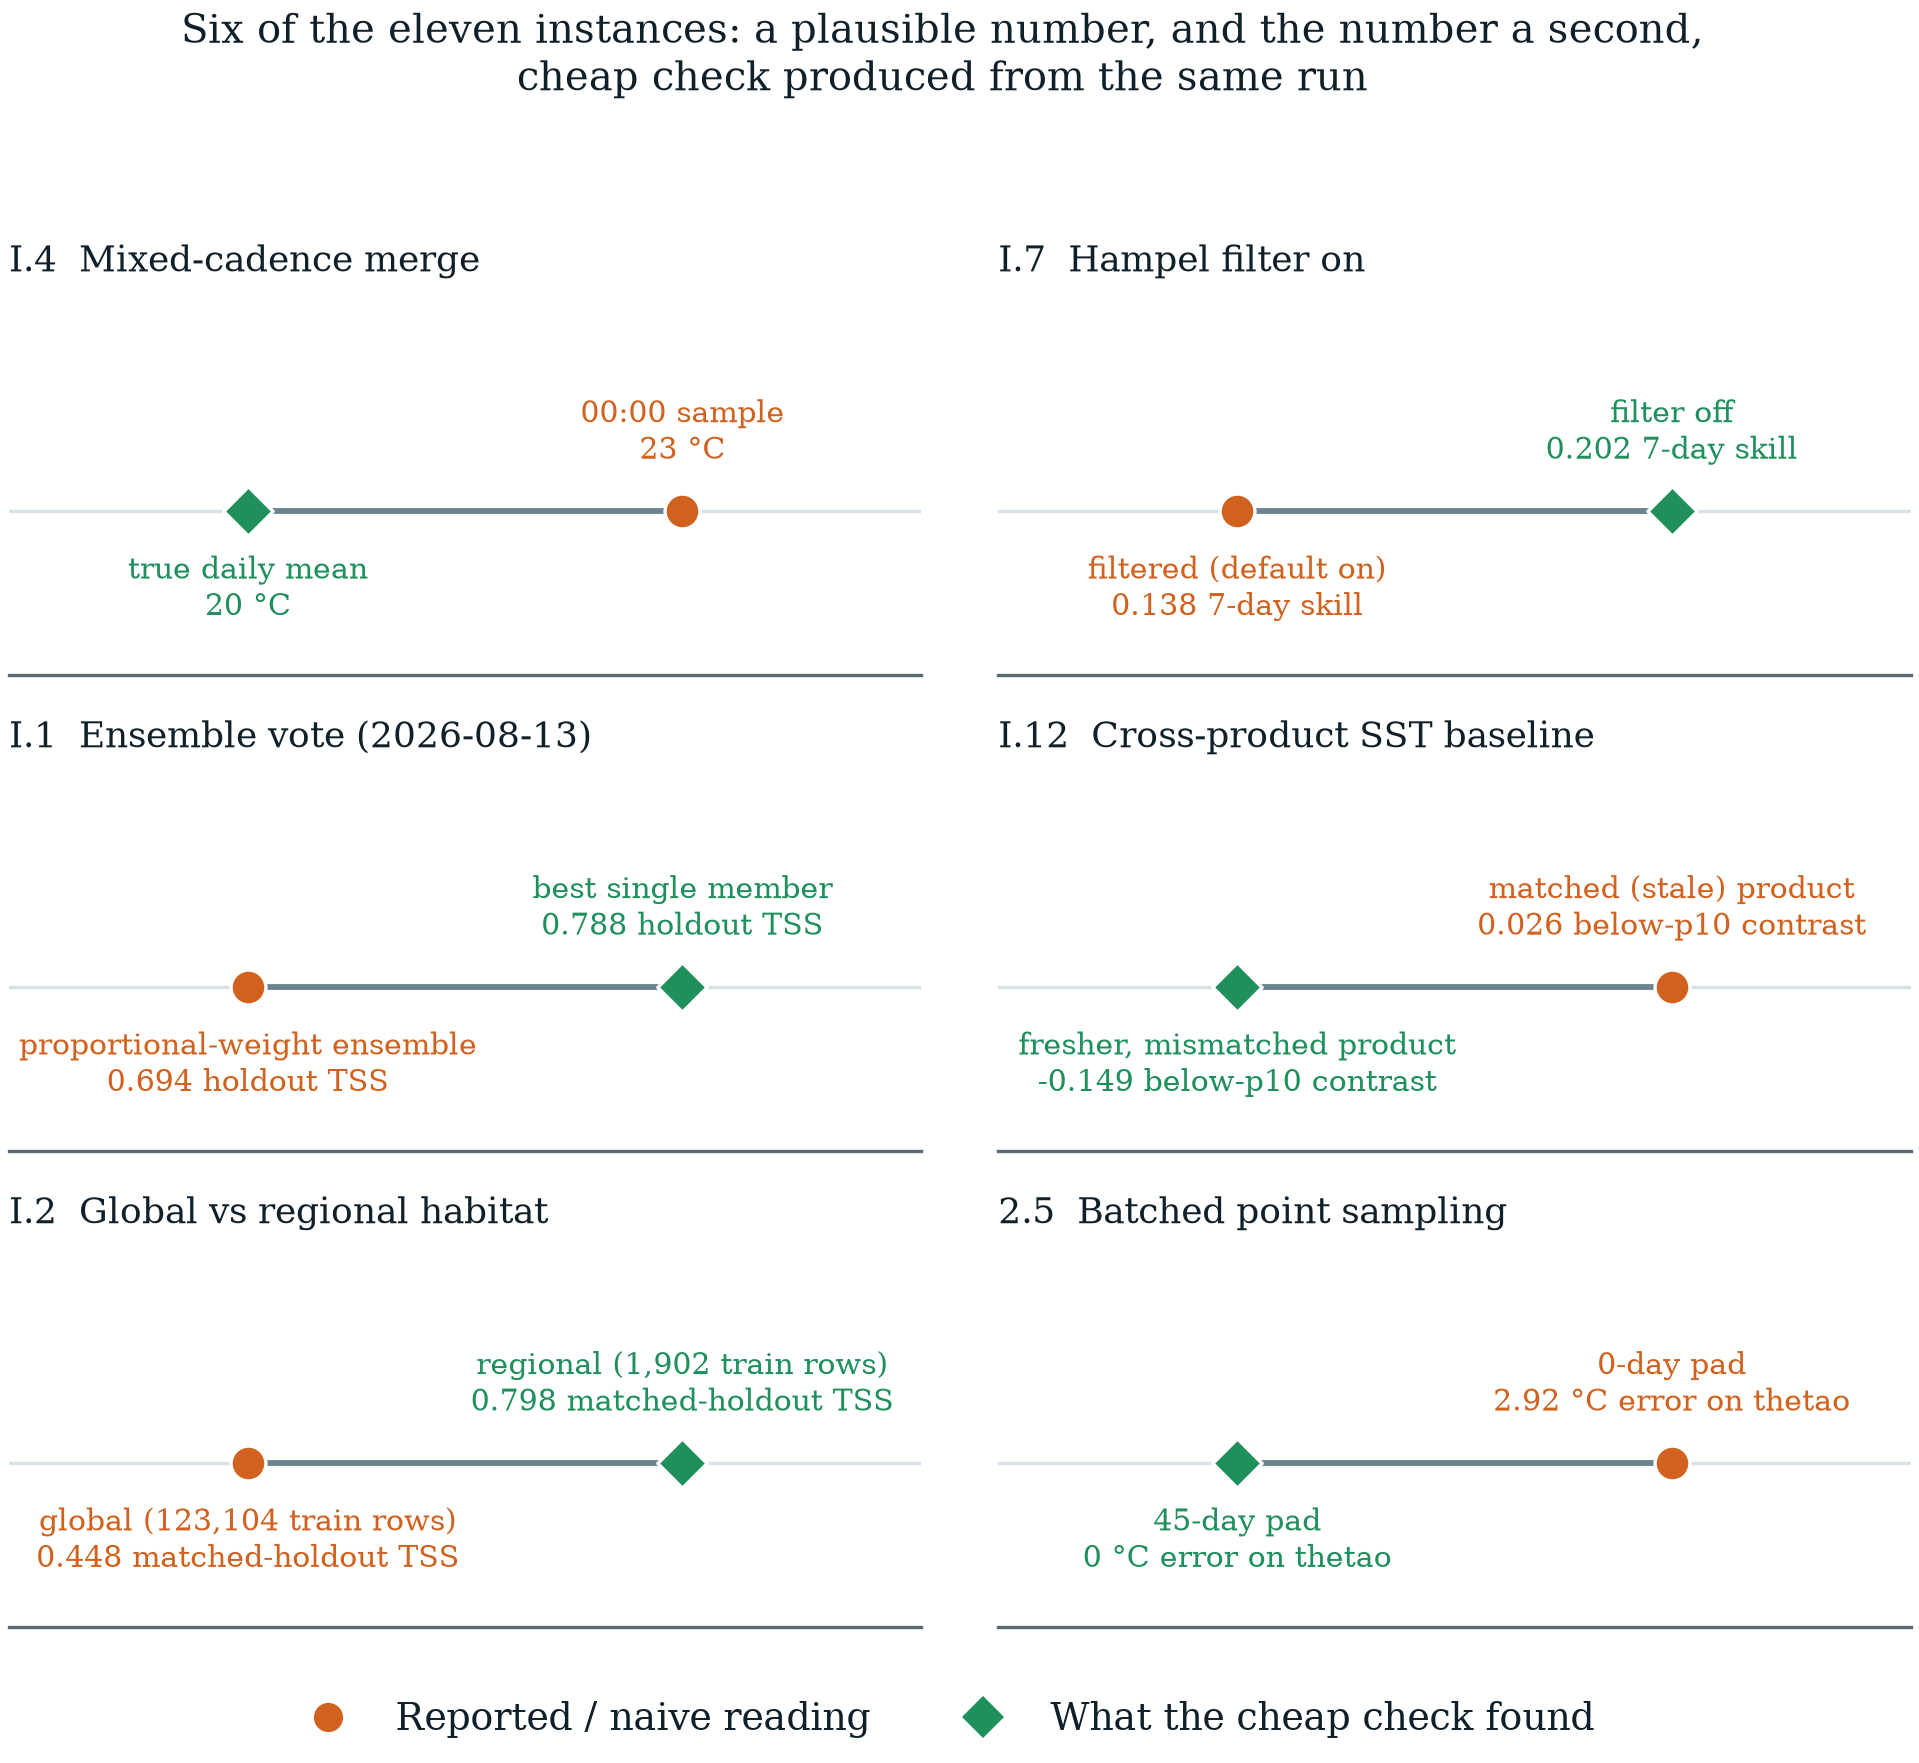
\includegraphics[width=0.92\linewidth]{naive_vs_checked}
\caption{Six of the eleven instances reduced to a single before/after number
pair: the reading that looked plausible on its own (orange circle) against
what a second, cheap check produced from the same run (green diamond). Units
differ by row; each panel has its own scale.}
\label{fig:naive}
\end{wfigure}

\section{Discussion}
\label{sec:discussion}

Read across all eleven, two patterns hold that neither instance alone would
establish. First, the direction is never neutral: every failure in this set
biased its host metric toward looking better, or at least more normal, than
the checked number shows it to be. A period mean read high rather than
scattering randomly around the true value; an ensemble's headline number
looked like an improvement; a detection count read as more complete than a
threshold-consistent detector can support; a fresher data product looked
like a strict upgrade. A failure that made a system look randomly wrong
would be caught by the first user who compared two runs. A failure that
makes it look plausible, or better, is caught only by whichever of the five
checks in \S\ref{sec:method} someone happens to run --- and Table
\ref{tab:instances}'s evidence column shows that even inside one team's own
codebase, most of those checks were run once, dated, and not committed as a
standing artifact.

Second, that observation applies to this paper's own evidence, not only to
the systems it describes, and two instances demonstrate it directly rather
than by analogy. Verifying I.2 for this paper meant re-reading the matched-
holdout comparison's own source file rather than trusting the companion
manuscript's macro, and the two disagreed: the companion manuscript states
the regional MaxEnt tier's TSS as 0.407, and the source file gives 0.365 ---
a transcription slip from spreadsheet to \LaTeX{} macro that nothing had
re-checked since the macro was written, because 0.407 is exactly as
plausible as 0.365 and neither is used elsewhere in that manuscript's
argument. It has been corrected in that manuscript's own build as a direct
consequence of applying, to this paper's own citations, the same discipline
\S\ref{sec:method} asks of the systems being studied. I.1 makes the same
point from a different angle: the 2026-08-13 measurement quoted in
\S\ref{sec:branch-b} is not a standing fact about the current model. Re-read
on \AsOf{}, MaxEnt's cross-validated TSS has since risen to
\EnsMaxentCVNow{} (from \EnsMaxentCVOld{}), narrowing the quality gap the
whole failure mode depends on, and the current ensemble weights it
accordingly (\EnsWeightLGBMNow{}\%/\EnsWeightRFNow{}\%/\EnsWeightMaxentNow{}\%
lightgbm/random forest/maxent). The mechanism the original measurement
demonstrated --- proportional weighting can score an ensemble below its own
best member --- still holds on an unrelated, more recent holdout, at a
much narrower margin (ensemble TSS \EnsHoldoutEnsembleNow{} against the
single best member's \EnsHoldoutBestNow{}), which is itself evidence the
effect's size is a direct function of the between-member quality gap it was
always claimed to depend on. Neither correction changes which of the eleven
instances is real; both show that a catalogue of silent, plausible,
signed-direction failures has to keep re-deriving its own numbers rather
than treating a prior write-up, including its own companion papers, as a
settled source.

\para{A practical checklist} The five checks in \S\ref{sec:method} are not
five different disciplines requiring five different tools --- they are five
answers to one question, asked of any number a pipeline is about to trust:
what would this number look like if it were wrong in the specific way this
computation could be wrong, and is that comparison actually run. A second
baseline answers it for "did the combination help." A control arm answers
it for "does the corroborating signal mean what it is being read to mean."
A hand-computed value against raw data answers it for "does the pipeline's
aggregate match what direct inspection shows." A synthetic fixture with a
known answer answers it for "is this transformation actually equivalent to
the one it replaced." An adversarial fixture answers it for "what does this
component do on an input built to break exactly this."

\section{Limitations}
\label{sec:limitations}

This is an instance catalogue from one system, assembled by the team that
built it, not a survey validated against an independent sample of ML
pipelines; the three-branch taxonomy in \S\ref{sec:results} is inductive
from these eleven and has not been tested against failures found elsewhere.
Most of the eleven were found while building or extending a feature, not
while auditing for bugs specifically, which is itself informative about base
rate but is not a controlled search and cannot support a claim about how
common this shape of failure is across the field. Five of the eleven
instances rest at least partly on a dated, single measurement rather than a
committed artifact: three (I.1, I.8's headline count, I.11) pair a headline
number that is a dated measurement of a moving state with a mechanism that
does have its own passing regression test, and two (I.7, I.12) are dated
throughout, with no committed test covering even the mechanism.
\S\ref{sec:method} and
Table~\ref{tab:instances} say which is which per instance rather than
averaging that uncertainty away, and a reader should weight the specific
numbers in those five accordingly. I.1 and I.2's fuller mechanism is documented in
companion papers cited rather than reproduced in full here; this paper's
contribution for those two is the cross-cutting frame, not new evidence
beyond what \S\ref{sec:discussion} adds.

\section{Conclusion}

Eleven instances from one operational marine machine-learning platform share
a shape: a component that is individually correct, well-tested, and
documented, feeding a downstream number that is real, computed from real
data, and licensed by convention to mean more than a second, cheap check
shows it to mean. None produced an exception; all biased their host metric
in the flattering direction. The checks that caught them --- a second
baseline, a control arm, a hand-computed reference, a synthetic case with a
known answer, an adversarial fixture --- cost little and are almost never
run by default. Two of this paper's own numbers drifted between when they
were first measured and when this paper verified them, which is not a flaw
in the argument but its clearest illustration: the discipline this paper
recommends for reading a pipeline's output has to be applied to a paper's
own citations, continuously, not once.


\section*{Reproducibility}
Every macro in \texttt{shared/generated/macros.tex} names its source file and
evidence grade inline; the figure is generated by
\texttt{generate\_figures.py} in this paper's \texttt{shared/} directory.
Every number below was verified against the file naming its source as of
\AsOf{}.
{\raggedright\sloppy
\begin{itemize}\itemsep1pt\parskip0pt
\item[] \textbf{Artifact (fully backed).} I.4, 2.5:
\texttt{backend/tests/\allowbreak{}test\_download\_cadence.py},
\texttt{machine\_learning/tests/\allowbreak{}test\_global\_sources.py}. I.5:
\texttt{backend/tests/\allowbreak{}test\_field\_sampling.py},
\texttt{backend/tests/\allowbreak{}test\_derived.py},
\texttt{backend/services/\allowbreak{}download/registry.py}. I.9:
\texttt{backend/services/\allowbreak{}field\_sampling.py},
\texttt{backend/tests/\allowbreak{}test\_forecast\_grid.py}. I.13:
\texttt{machine\_learning/reports/\allowbreak{}hab\_early\_warning\_*\_summary.json}
and matching \texttt{*\_holdout.csv} for all five regions. I.2
(re-verified \AsOf{}): \texttt{machine\_learning/reports/\allowbreak{}global\_vs\_regional\_habitat.csv};
I.2's full mechanism is \texttt{machine\_learning/scripts/\allowbreak{}validate\_global\_on\_region.py}
\citep{moredata2026}.
\item[] \textbf{Artifact + dated (tested mechanism, dated headline).} I.1:
mechanism and current re-verification (\AsOf{}) in
\texttt{machine\_learning/reports/\allowbreak{}fish\_habitat\_summary.json},
\texttt{fish\_habitat\_holdout.csv}; 2026-08-13 headline figures in
\texttt{machine\_learning/fish\_habitat\_prediction/\allowbreak{}src/models.py}.
I.8: mechanism tests in \texttt{backend/tests/\allowbreak{}test\_eddies.py};
dated count in \texttt{backend/services/\allowbreak{}eddies.py}. I.11:
mechanism test in \texttt{backend/tests/\allowbreak{}test\_upwelling.py};
dated corroboration rates in \texttt{backend/services/\allowbreak{}upwelling.py}.
\item[] \textbf{Dated (no committed artifact).} I.7:
\texttt{backend/forecasting/\allowbreak{}preprocessing.py}. I.12:
\texttt{backend/services/\allowbreak{}sst\_anomaly.py}, naming
\texttt{scripts/measure\_sst\_corroboration.py} and
\texttt{scripts/build\_climatology\_copernicus.py}.
\end{itemize}}

\bibliographystyle{IEEEtran}
\bibliography{../shared/references}

\end{document}
